\documentclass[10pt, a4paper]{beamer}
\usepackage{graphicx} % For including images
\usepackage{caption}  % For \captionof{figure}
%\documentclass{article}

\usepackage{hyperref}

%Metadaten
\title{Threat and Weakness Analysis in SimplyTag}

\subtitle{ORGADATA COMPANY, LEER}
\newcommand{\additionalsubtitle}{Data Science} 
\author{
	Manoj Selvaraju - 7025649 \\ 
	Vatsal Mahajan - 7025694\\ 
	Vijay Singh - 7025700
}

%\date{\today}
\date{January 15, 2025}

% siehe hesader.tex Zeile 10-16 zum Aktivieren der Notes
% Kommentare stehen in \notes{} und können im 2-screen-mode genutzt werden
%%%%%%
%
% $Autor: Wings $
% $Datum: 2020-01-18 11:15:45Z $
% $Pfad: githubtemplate/Template/Presentations/Template/slides/header.tex $
% $Version: 4620 $
%
%
% !TeX encoding = utf8
% !TeX root = Rename
%
%%%%%%


%Packages
\usepackage[utf8]{inputenc} %Für Umlaute, da BibLaTeX
\usepackage[english]{babel}
\usepackage{amsmath}
\usepackage{amsfonts}
\usepackage{amssymb}
\usepackage{colortbl}
\usepackage{cancel} %'\cancel{}', '\bcancel{}' und '\xcancel{}'

%%%%%%%%%2-Screen%%%%%%%%%%%%%%%%%%%%%%%%%%%%%%%%%%%%%%%%%%%%
\usepackage{pgfpages} 
%%%%Kommentiert für Beamer
%%%%Aktiv für Notes
%\setbeameroption{show notes on second screen=bottom}
%\setbeameroption{second mode text on second screen=bottom}
%%%%%%%%%%%%%%%%%%%%%%%%%%%%%%%%%%%%%%%%%%%%%%%%%%%%%%%%%%%%%

%Für Grafiken
\usepackage{tikz}
\usetikzlibrary{mindmap}
\usepackage{gnuplottex}
\usepackage{pgf}
\usepackage{colortbl} 
\usetikzlibrary{calc}
\usetikzlibrary{shapes,arrows} %Für Flowchart
\usetikzlibrary{shapes.geometric} %Für Flowchart
\usepackage{scalefnt}
\usetikzlibrary{decorations.markings} %Für => pfeile
\usetikzlibrary{calc,patterns,decorations.pathmorphing,decorations.markings}
%Für urls in Quellen
\usepackage{url}
%Für Diagramme (autotools)
%\usepackage{graphicx}
%\usepackage{graphviz}

%\usepackage[
%  backend=biber,
%  style=alphabetic,
%  sorting=ynt
%]{biblatex}

\usepackage[natbib=true,style=alphabetic,backend=bibtex,useprefix=true]{biblatex}

%Formatierungen
\mode<presentation>
\setbeamertemplate{headline} 
{%
\begin{beamercolorbox}[rounded=true, center]{bgcolor}
\begin{columns}[T]
\begin{column}{9cm}
{\color{gray}\begin{tiny}Hochschule Emden/Leer\end{tiny}} \\ 
{\color{gray}\begin{tiny}Department of Electrical Engineering and Computer Science\end{tiny}} \\ 
{\color{gray}\begin{tiny}Industrial Informatics\end{tiny}} \\
%{\color{gray}\begin{tiny}Innovationsforum MSR\end{tiny}}
\end{column}
\begin{column}{2cm}

\includegraphics[scale=0.25]{img/technik.jpg}
\end{column}
\end{columns}
\end{beamercolorbox}
 }
\insertsectionhead
\insertsubsectionhead
\usetheme{default}
\useinnertheme[shadow=true]{rounded}
\usebackgroundtemplate
{%
      \rule{0pt}{\paperheight}%
      \hspace*{\paperwidth}%
      \makebox[0pt][r]{
\includegraphics[width=\paperwidth]{img/hintergrund2.png}}
 }

\definecolor{HSELhellblau}{RGB}{138,198,203}
\definecolor{HSELblau}{RGB}{0,59,95}
\usecolortheme[named=HSELblau]{structure}
 \newcommand{\topline}{%
  \tikz[remember picture,overlay] {%
    \draw[HSELhellblau] ([yshift=-0.9cm]current page.north west)
             -- ([yshift=-0.9cm,xshift=\paperwidth]current page.north west);}}
\setbeamertemplate{section}[numbered]


\newcommand{\STANDARD}[2]
{
  \mode<presentation>%
  {%
     \begin{frame}[allowframebreaks]{#1} #2 \end{frame}
  }%
  \mode<article>
  {
    \fcolorbox{AliceBlue}%{Bisque} %{BlanchedAlmond}
    {LightGrey} %{Beige}   %{AliceBlue}
    {
      \begin{minipage}{\textwidth}{\bf #1} #2  \end{minipage}
      
      
    }%
    
    \medskip
    \hrulefill
  }
}

\newcommand{\MYNOTE}[1]
{
  \mode<presentation>%
  {%
     %\note{#1}
     \only<article>{#1}
  }%
  \mode<article>
  {
    #1
  }
}

% ------------
% sectionframe
% ------------
%
% #1  Der Name der section.
%
\newcommand{\sectionframe}[1]%
{%
	\begin{frame}
		\Huge
		\begin{center}
			#1 
		\end{center}
	\end{frame}%
}

\newcommand{\Mysection}[1]%
{%
  \section{#1}%
  
  \sectionframe{#1}%
}

\usepackage{listings}

% Farben für Syntax-Highlighting
\definecolor{dkgreen}{rgb}{0,.6,0}
\definecolor{dkblue}{rgb}{0.655,0.113,.364}
\definecolor{dkyellow}{cmyk}{0,0,.8,.3}

\definecolor{parameterc}{rgb}{.4,0,.6}
\definecolor{typec}{rgb}{0,0.525,.702}
\definecolor{stringc}{rgb}{0,.5019,.5019}
\definecolor{keywordc}{rgb}{.6549, .1137, .3647}
\definecolor{commentc}{rgb}{.5882, .5960, .5882}
\definecolor{textc}{rgb}{.2,.2,.2}

\lstdefinestyle{all}{
	alsoletter={-},
	frame=single, 	% top,frame=bottom,
	numbers=none,
	numberstyle=\tiny\color{textc},
	basicstyle=\linespread{0.9}\ttfamily\footnotesize\color{textc},
	tabsize=4,
	showstringspaces=false,
	captionpos=t,
	rulecolor=\color{lightgray!40},
	keywordstyle=\color{keywordc},
	stringstyle=\color{stringc},
	commentstyle=\color{commentc},
	breaklines=true,
	escapechar="!",
	postbreak=\mbox{\textcolor{green}{$\hookrightarrow$}\space},
}

\lstdefinestyle{bashstyle}{
	style=all,
	keywords=[2]{-y, --no-install-recommends, --allow-change-held-packages, --allow-downgrades, --fetch-keys, -n, --version, --params, -c, -i, -O, --upgrade, --no-cache-dir, --extra-index-url, --show, -s, -m},
	keywordstyle=[2]\color{parameterc},
	morekeywords = {ln,choco,pip,pip3,apt,apt-key,apt-get,apt-mark,add-apt-repository,wget,mktemp,dpkg,dpkg-query,echo,>>,rm,tegrastats, systemctl},
	deletekeywords={local,LOCAL},
}

\lstdefinestyle{pythonstyle}{
	style=all,
	morekeywords={as},
	keywords=[2]{True, False, None},
	keywordstyle=[2]\color{typec},
	alsoletter={_},
	keywords=[3]{max_workspace_size_bytes, precision_mode, maximum_cached_engines, use_calibration, optimizer, loss, input_shape, from_logits, metrics, batch_size, epochs, validation_data, activation, use_calibration, filters, kernel_size, pool_size, units},
	keywordstyle=[3]\color{parameterc},
	deletekeywords={compile,COMPILE},
}

\lstdefinestyle{inlinestyle}{
	style=all,
	breaklines        = true,
	breakatwhitespace = true,
	breakindent       = 2ex,
	escapechar        = *,
	numbers           = left,
	postbreak=,
}
\lstdefinelanguage{MyBash} {
	language = Bash,
	style=bashstyle,
}

\lstdefinelanguage{MyPython} {
	language = Python,
	style=pythonstyle,
}


\definecolor{PythonColor}{rgb}{0,0.5,1.}
\newcommand{\PYTHON}[1]{\textcolor{PythonColor}{\texttt{#1}}}
\definecolor{PythonColorHighLite}{rgb}{0.5,0,1.}
\newcommand{\PYTHONHL}[1]{\textcolor{PythonColorHighLite}{\texttt{#1}}}
\definecolor{MapleColor}{rgb}{1,0,0}
\newcommand{\MapleCommand}[1]{\textcolor{MapleColor}{\texttt{#1}}}
\definecolor{ShellColor}{rgb}{0,1,1.}
\newcommand{\SHELL}[1]{\textcolor{ShellColor}{\texttt{#1}}}
\definecolor{FileColor}{rgb}{1,0,1.}
\newcommand{\FILE}[1]{\textcolor{FileColor}{\texttt{#1}}}


%\addbibresource{Documents/MyLiterature.bib} %Import the bibliography file

\begin{document}
	
	
\setbeamercolor{bgcolor}{fg=black,bg=white}
\selectlanguage{English}
\setbeamertemplate{footline}{%
\vspace*{-.1cm}\hspace*{.5cm}
\scriptsize{%
%%\hspace*{1pt}\insertauthor
%%\inserttitle
\hspace{325pt}\insertframenumber/\inserttotalframenumber}
}

\STANDARD{}
{
  \titlepage
}

\MYNOTE
{
  \ldots
}



\STANDARD{Table of Content}
{
\tableofcontents
}

\MYNOTE
{
  \ldots
}

\setbeamercovered{transparent}

	
	
	%%% Vijay's content, last me conclusion add krna mt bhul na.
	
	\section{Introduction}
	\begin{frame}
		\frametitle{Introduction}
		
		\begin{block}{About ORGADATA:}
			\begin{itemize}
				\item Orgadata is a leading software company, specializing in solutions for window and door digitalization, offering services like SimplyTag.
				\item SimplyTag is a tool that provides quick and convenient access to construction-related data for specific elements (e.g., windows or doors) using QR codes, enabling on-site professionals to retrieve essential information in real time.
			\end{itemize}
		\end{block}
		
		\begin{block}{Why?}
			\begin{itemize}
				\item As a student of Industrial Informatics, we have studied how to digitalize products and processes in line with Industry 4.0 principles.
				\item In today’s digital age, safeguarding sensitive information and system integrity is crucial.
				\item Threat and Weakness Analysis is an essential step in mitigating risks, preventing breaches, and ensuring operational resilience.	
			\end{itemize}
		\end{block}
		
	\end{frame}
	
	
	
	\section{Purpose of Analysis}
	\begin{frame}
		\frametitle{Purpose of Analysis}
		
		\begin{block}{}
			\begin{itemize}
				\item Exploit exposed endpoints or unauthorized access.
				\item Detecting vulnerabilities in Orgadata's systems that could be exploited by malicious actors.
				\item Prevent unauthorized access attempts.
				\item Improve data security by safeguarding sensitive information of customer and operational data against breaches.
				\item Build a predictive model using the KDD process to classify threats and evaluate system requests effectively.
				\item Provide actionable insights to enhance system security and performance.
			\end{itemize}
		\end{block}
		
	\end{frame}
	
	
\section{Challenges}
\begin{frame}
	\frametitle{Challenges We Faced}
	
	\begin{block}{}
		\begin{itemize}
			\item Understanding the huge data (approx. 2.2 million rows) provided in `.log` file and JSON formats.
			\item Distinguishing between genuine user activities and malicious attempts.
			\item Handling complex patterns in user behavior and request logs.
		\end{itemize}
	\end{block}
	
	\centering
	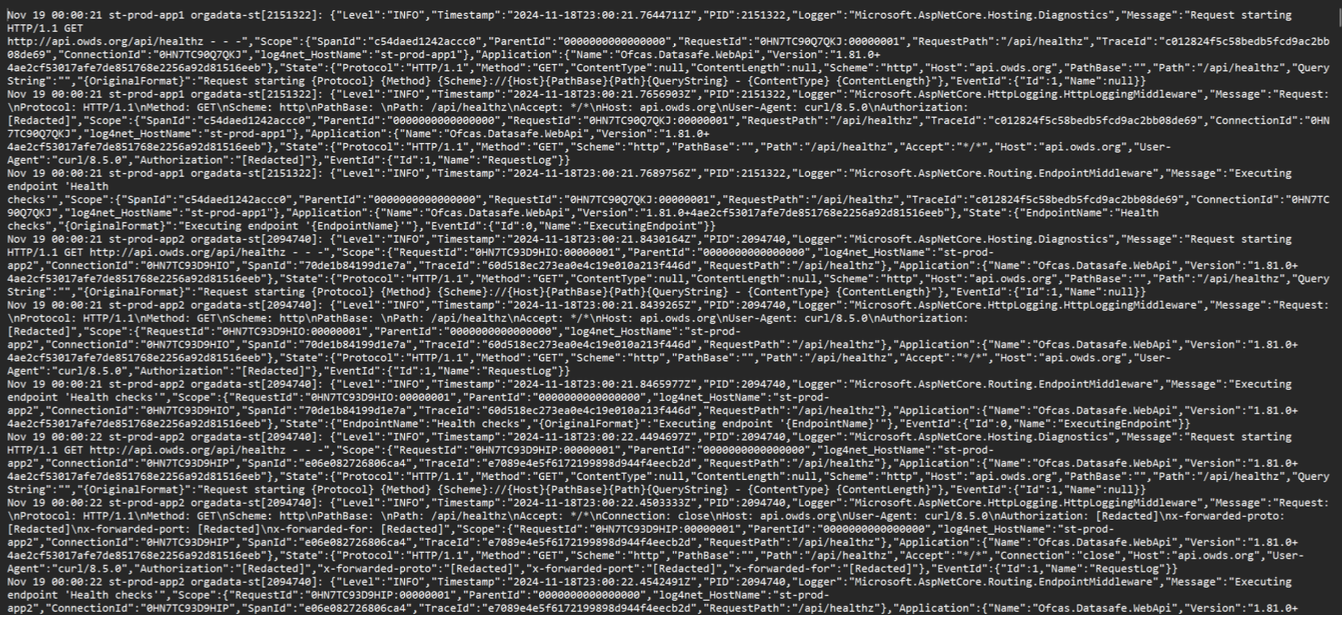
\includegraphics[width=0.8\textwidth]{images/LogSS.png} % Adjust width as needed
	\centering
	\captionof{figure}{1.Raw Log Data}
	
\end{frame}


\section{Application Sector}
\begin{frame}
	\frametitle{Application Sector}
	This project belongs to the Industry Domain, specifically for the Digital Tools and Software Solutions domain, with a focus on:
	
	\begin{block}{}
		\begin{itemize}
			\item Threat Detection
			\item Data Integrity Assurance
			\item Operational Security Optimizations
			\item Cybersecurity Measures
		\end{itemize}
	\end{block}
\end{frame}

\section{Positioning Analytics in Relevant Architectures}
\begin{frame}
	\frametitle{Positioning Analytics in Relevant Architecture}
The analytics focus on cybersecurity and anomaly detection, aligning with ISO standards for secure data handling and reliable operations.

	
	\begin{block}{}
		\begin{itemize}
		\item \textbf{RAMI 4.0:} Positioned in the Information Layer (real-time data collection, processing and analysis for threat detection).
		\item \textbf{IIRA:} Located in the Control Domain (automated threat detection and response) and the Operations Domain (long-term system optimization and strategic planning).
		\end{itemize}
	\end{block}
	
		% Image placed below
	\centering
	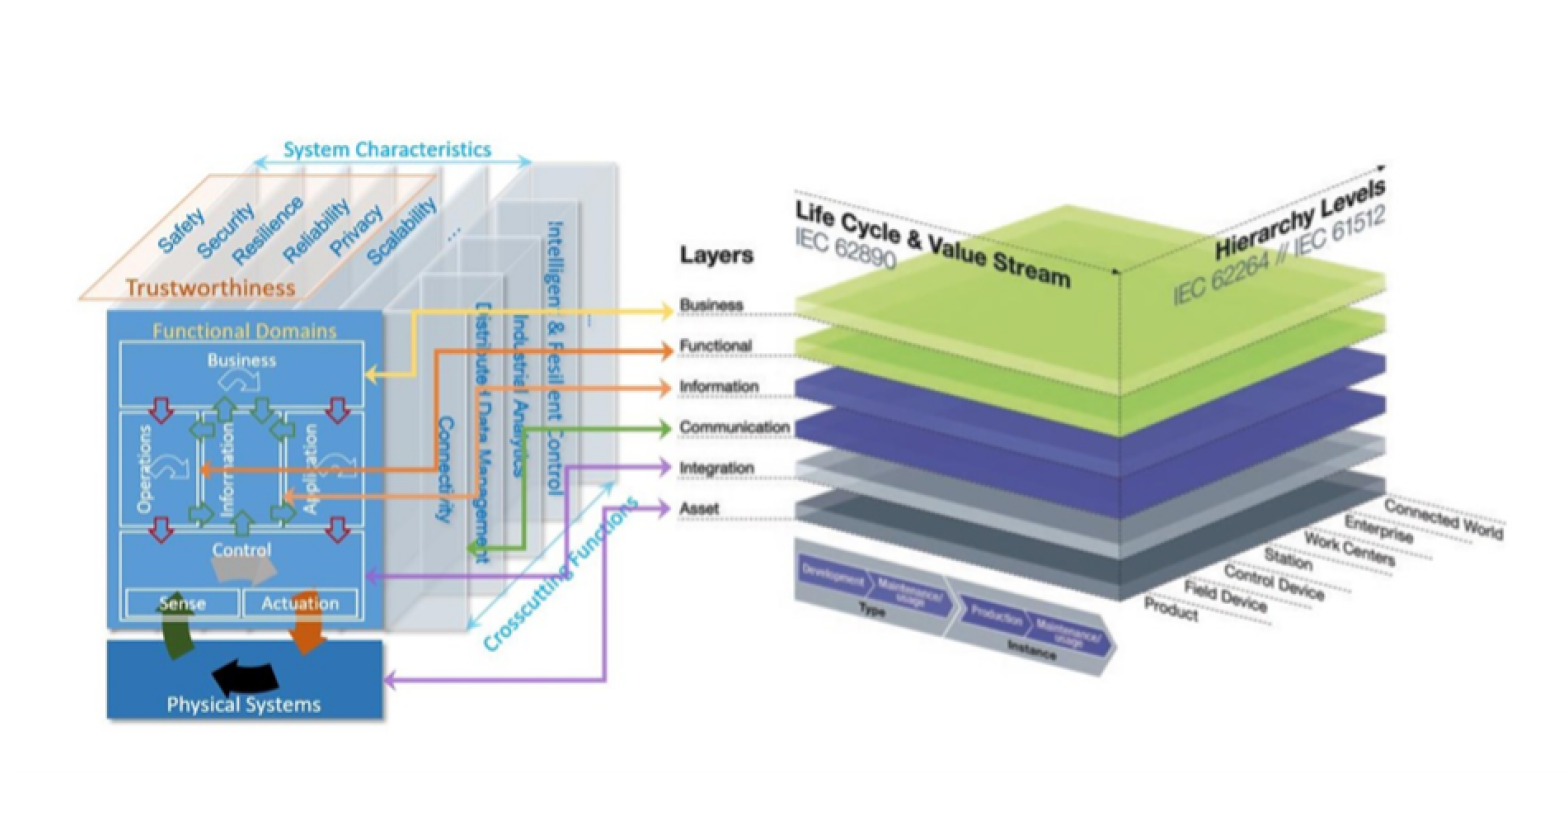
\includegraphics[width=0.6\textwidth]{images/RAMI_IIRA.png} % Adjust width as needed
	
	% Add image name below
	\centering
	\captionof{figure}{2.RAMI\_IIRA}
	
	
\end{frame}

	
	
\section{Knowledge Discovery in Database (KDD) Process}
\begin{frame}
	\frametitle{Knowledge Discovery in Database (KDD) Process}
	\begin{block}{Data Selection:}
		Identify and Extract relevant data from log files while filtering out irrelevant information.
		\begin{itemize}
			\item \textbf{Data Origin:} \textit{Graylog server} 
			\item \textbf{Format:} \textit{.log} 
			\item \textbf{Size:} 3.34 GB
			\item \textbf{Features:} Timestamps, PID, Logger, Message, Scope (e.g., TraceId, RequestID), Application, State, EventID.
		\end{itemize}
	\end{block}
	
	% Image placed below
	\centering
	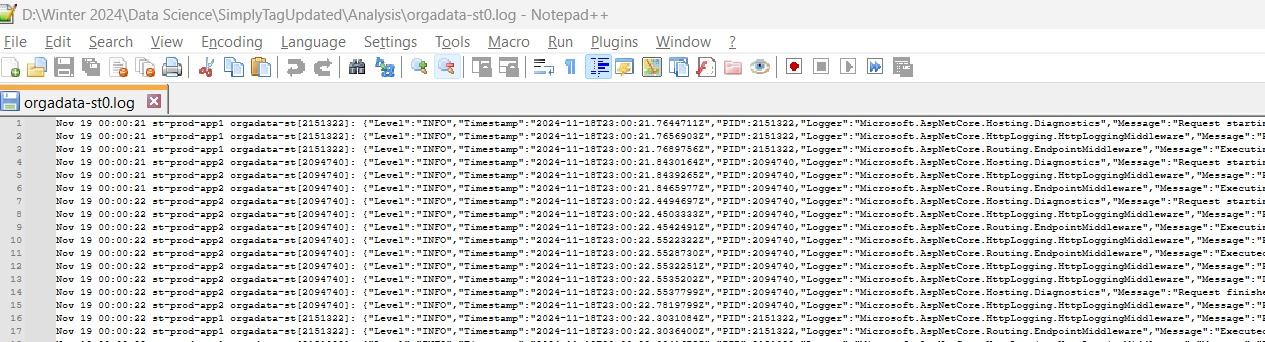
\includegraphics[width=0.9\textwidth]{images/Database.jpeg} % Adjust width as needed
	
	% Add image name below
\centering
	\captionof{figure}{3.Database}
	
\end{frame}


	
	\begin{frame}
		\frametitle{Data Preparation:} 
		Given the dataset, the following steps are carryout out to make the dataset clean and ready for analysis
		\begin{block}{}
			\begin{itemize}
				\item \textbf{Merging and Conversion:} Format .log to CSV
				\item \textbf{Cleaning:} Removed entries with no traceid, errors ,warnings
				\item \textbf{Identified Key Attributes:} Trace-ID, Status code, Path and User Agent
			\end{itemize}
		\end{block}
		
		
				% Image placed below
		\centering
		\includegraphics[width=1\textwidth]{images/csvFIle.png} % Adjust width as needed
		
		% Image name below the image
		\vskip 0.1cm % Adds a bit of vertical space between image and text
		\centering
		\captionof{figure}{4.CSV File}
		
	\end{frame}
	
	
	
	\begin{frame}
		\frametitle{Data Transformation}
		\begin{block}{}
			Restructure and manipulate the cleaned data for analysis.
			\begin{itemize}
				\item Grouped log entries by TraceId to rebuild complete request flows
				\item Parsed fields from nested JSON structures: TraceId, HTTP Status Code, Path, User-Agent.
				\item Transformed each log entry into a distinct row, aligning TraceId with its corresponding attributes for seamless analysis.
			\end{itemize}
		\end{block}
		
		% Add vertical space
		\vfill
		
		% Image placed below
		\centering
		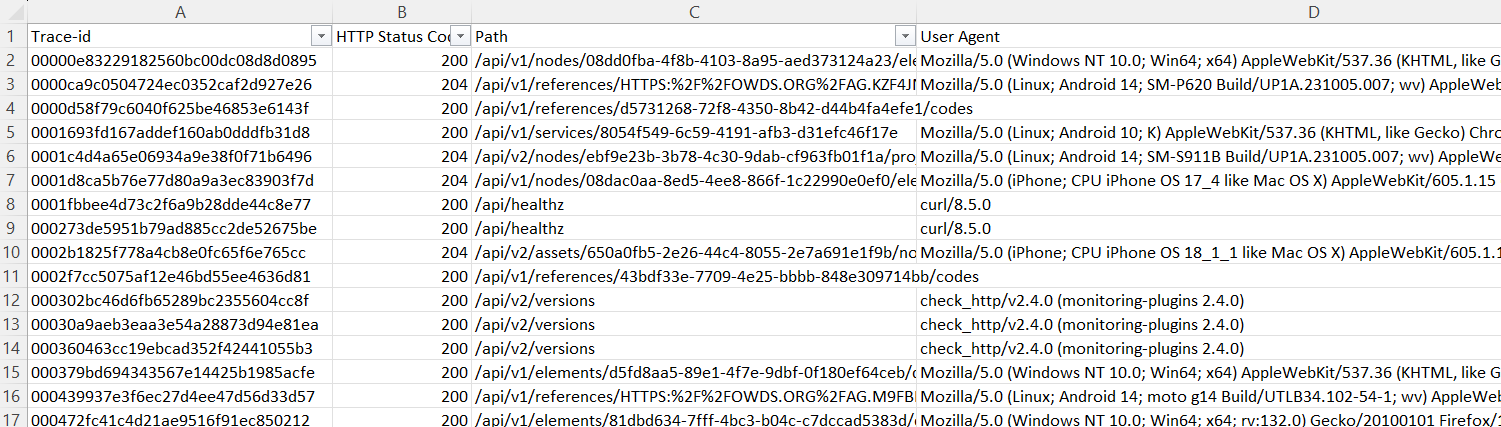
\includegraphics[width=1\textwidth]{images/DataTransformation.png} % Adjust width as needed
		
		% Image name below the image
		\vskip 0.1cm % Adds a bit of vertical space between image and text
		\centering
		\captionof{figure}{5.Transformed CSV data}% You can replace this with the actual name of the image
	\end{frame}
	
	\begin{frame}
		\frametitle{Data Mining}
		
		\begin{block}{Feature Extraction}
			Extracted hidden patterns and anomalies from the selected data.
			\begin{itemize}
				\item \textbf{Path-Based Features (Approach 1 \& 2):}
				\begin{itemize}
					\item Extracted key features based on the Path attribute. Features included:
					\begin{itemize}
						\item \textbf{Path length}
						\item \textbf{Presence of special characters}
						\item \textbf{SQL keywords}
						\item \textbf{Path traversal attempts}
						\item \textbf{Suspicious file extensions}
					\end{itemize}
					\item Applied TF-IDF vectorization on the Path attribute to convert API endpoint access into numerical features for machine learning.
				\end{itemize}
				
				\item \textbf{User-Agent Analysis (Approach 3):}
				\begin{itemize}
					\item Analyzed User-Agent strings to detect patterns linked to suspicious or malicious activities.
				\end{itemize}
			\end{itemize}
		\end{block}
	\end{frame}
	

	
	\begin{frame}
		\frametitle{Data Mining}
		
		\begin{block}{Clustering and Anomaly Detection}
			
			\begin{itemize}
				\item \textbf{Approach 1:} Path and Frequency-Based Clustering
				\begin{itemize}
					\item Combined extracted path features with frequency metrics and HTTP status codes.
					\item Used \textbf{DBSCAN} for clustering and \textbf{Isolation Forest} for outlier detection.
				\end{itemize}
				\item \textbf{Approach 2:} TF-IDF and Clustering
				\begin{itemize}
					\item Utilized TF-IDF vectorized features and numeric attributes for clustering.
					\item Integrated \textbf{DBSCAN} and \textbf{Isolation Forest} for robust anomaly detection, flagging unusual requests.
				\end{itemize}
				
				\item \textbf{Approach 3:} User-Agent Pattern Analysis
				\begin{itemize}
					\item Focused on identifying suspicious behaviors using \textbf{User-Agent} patterns.
				\end{itemize}
			\end{itemize}
		\end{block}
		
	\end{frame}

	\begin{comment}	
	\begin{frame}
		\frametitle{Data Modelling}
		Used Unsupervised learning to perform clustering and anomaly detection
		
		\begin{columns}
			% Left column for DBSCAN
			\column{0.5\textwidth}
			\begin{block}{Model 1: DBSCAN}
				\begin{itemize}
					\item \textbf{Purpose:} Group data points based on density; flag points that don’t belong to any cluster as anomalies.
				\end{itemize}
				\begin{itemize}
					\item \textbf{Key Parameters:}
					\begin{itemize}
						\item \textbf{eps: 0.5}
						\item \textbf{min\_samples: 5}
					\end{itemize}
				\end{itemize}
				\begin{itemize}
					\item \textbf{Outcome:} Requests not assigned to any cluster (cluster = -1) were flagged as anomalies.
				\end{itemize}
			\end{block}
			
			% Right column for Isolation Forest
			\column{0.5\textwidth}
			\begin{block}{Model 2: Isolation Forest}
				\begin{itemize}
					\item \textbf{Purpose:} Detect anomalies by isolating data points, as anomalies are easier to separate from the rest of the data.
				\end{itemize}
				\begin{itemize}
					\item \textbf{Key Parameters:}
					\begin{itemize}
						\item \textbf{n\_estimators: 100} 
						\item \textbf{contamination: 0.01}
						\item \textbf{random\_state: 42}
					\end{itemize}
				\end{itemize}
				\begin{itemize}
					\item \textbf{Outcome:} Anomalous requests were flagged with a value of -1.
				\end{itemize}
			\end{block}
		\end{columns}
	\end{frame}
	
	\end{comment}	
	
	
	
	\begin{frame}
		\frametitle{}
		\begin{block}{Validation/ Verification}
			\begin{itemize}
				\item \textbf{DBSCAN:} Verified datapoints within clusters had similar patterns and the endpoints with SwaggerUI
				\item \textbf{Isolation Forest:} Distribution of anomaly scores was evaluated to differentiate anomalies from regular requests.
			\end{itemize}
		\end{block}
		
		\begin{block}{Data Visualization}
			
		\begin{minipage}{0.48\textwidth}
			\centering
			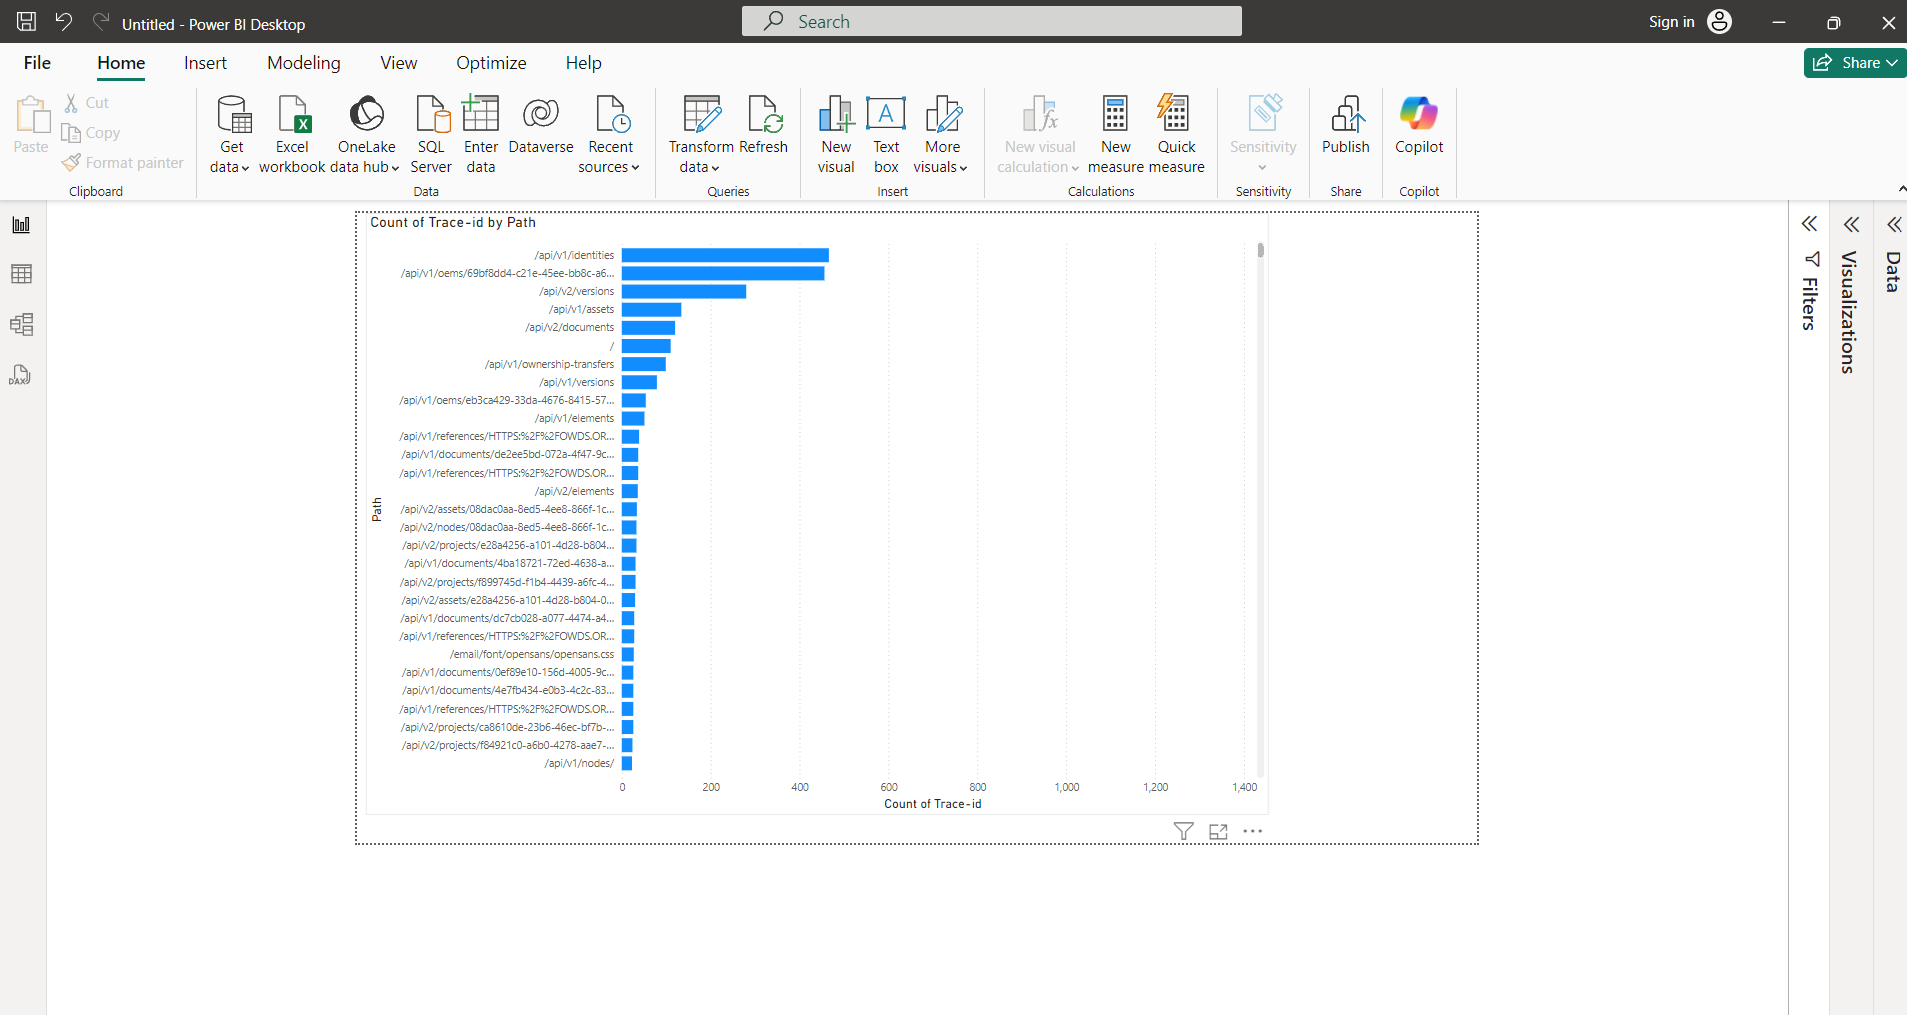
\includegraphics[width=\textwidth]{images/PowerBI_1.png}
			\captionof{figure}{6.Analysis based on Path}
		\end{minipage}
		\hfill
		\begin{minipage}{0.48\textwidth}
			\centering
			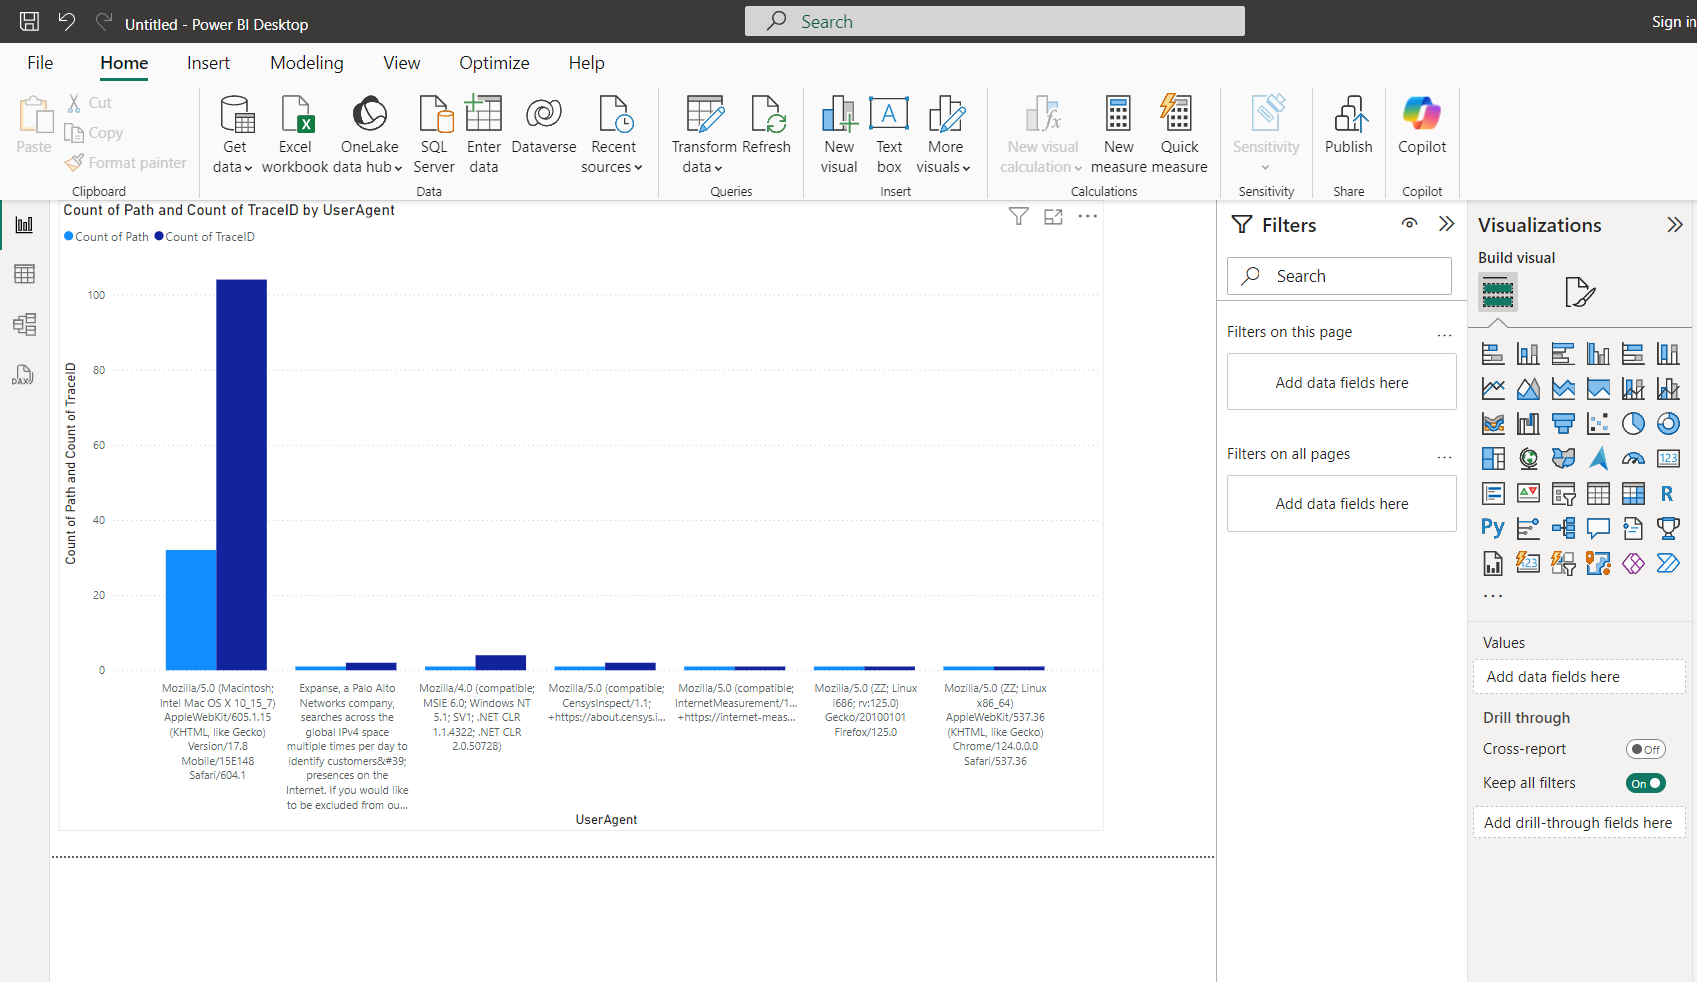
\includegraphics[width=\textwidth]{images/PowerBI_2.png}
			\captionof{figure}{7.Analysis based on Useragent}
		\end{minipage}
		
			\end{block}
		\end{frame}
	
	
	\section{Conclusion and Future Scope}
	\begin{frame}
		\frametitle{Conclusion and Future Scope}
		
		\begin{block}{Conclusion:}
			\begin{itemize}
				%\item Successfully analyzed Orgadata’s SimplyTag log files using the Knowledge Discovery in Databases (KDD) process to identify potential threats
				\item Used Knowledge Discovery in Databases (KDD) process to identify potential threats.
				\item Applied machine learning techniques like DBSCAN and Isolation Forest for clustering and anomaly detection.
				\item Found exposed endpoints or unauthorized access requests.
			\end{itemize}
		\end{block}
		
				\begin{block}{Future Scope:}
			\begin{itemize}
				\item Unified Approach Integration
				\item Advanced Model Optimization Algorithms
				\item Automated Feature Engineering	
				\item Broader Dataset Analysis			
			\end{itemize}
		\end{block}
	
	\end{frame}
	
	
	
	
	
	\STANDARD{}
{
  \begin{columns}
    \begin{column}{0.35\textwidth}
      \begin{block}{~~~~~~Thank you}
        \centering
        for your attention
      \end{block}
    \end{column}
  \end{columns}
}

\MYNOTE{Ja, \textbf{Vielen} Dank, für Ihre Aufmerksamkeit}


	
\end{document}
